\documentclass[12pt,a4paper,twoside]{article}
\usepackage[pdfborder={0 0 0}]{hyperref}
\usepackage[margin=25mm]{geometry}
\usepackage{pdfpages}
\usepackage{graphicx}
\usepackage{parskip}
\begin{document}

%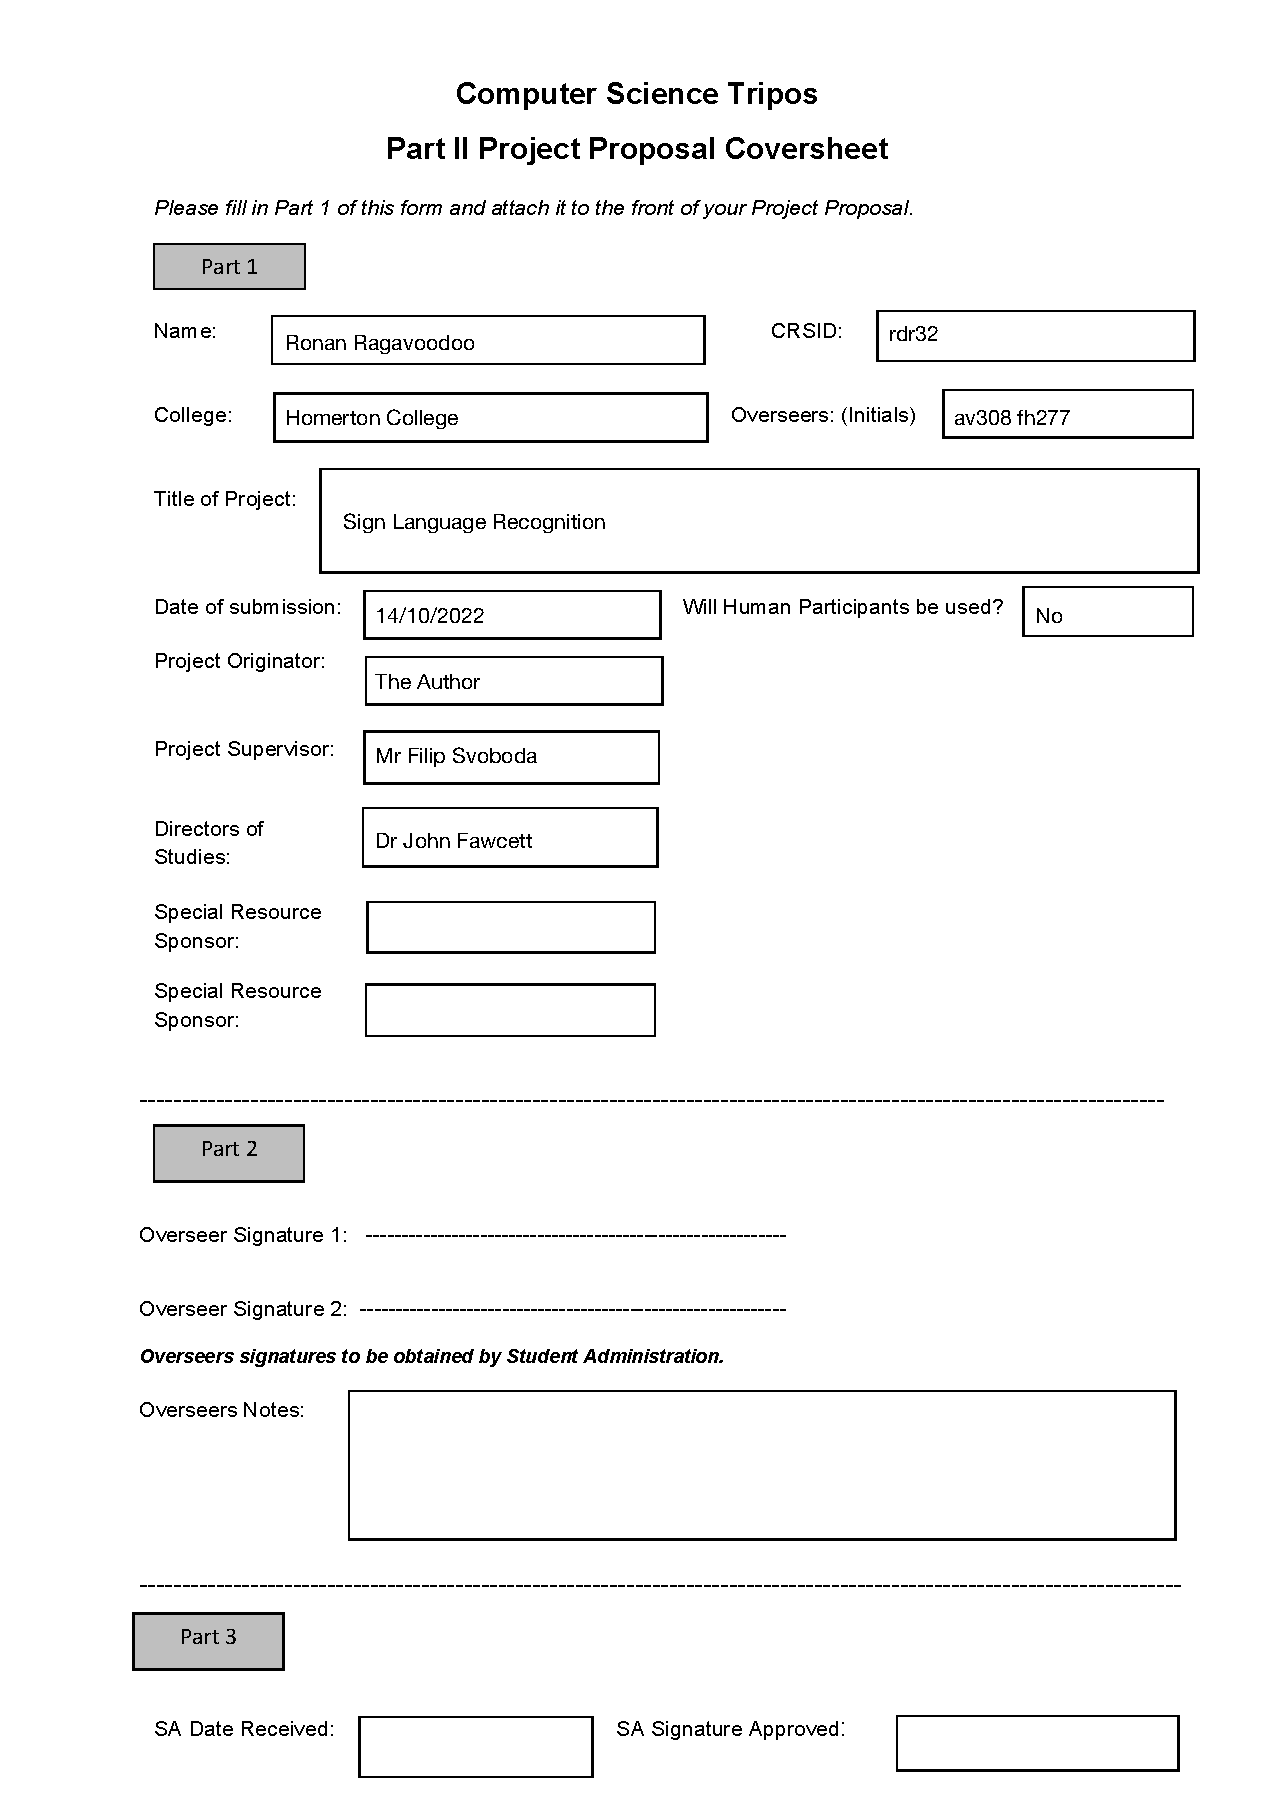
\includepdf[pages={1}]{proposalform.pdf}

\begin{center}
    \Large
    Computer Science Tripos -- Part II -- Project Proposal\\[4mm]
    \LARGE
    Sign Language Recognition\\[4mm]

    \large
    Dissertation Author

    Originator: The Author

    14 October 2022
\end{center}

\vspace{5mm}

\textbf{Project Supervisor:} Mr. Filip Svoboda

\textbf{Director of Studies:} [Redacted for Blind Grading]

\textbf{Project Overseers:} Dr. Ferenc Huszar \& Dr. Andreas Vlachos

\textbf{University Teaching Officer:} Professor Nicholas Lane

% Main document

\section*{Introduction}

Sign Language has been adopted by many people who are unable to speak, or hear. While technology has been used to help this affected minority group to a certain degree, there are still a lot of facilities that can be improved to help them communicate. For example, even Windows does not support a form of sign language recognition. This is  despite the advances that we have concerning digital assistants, which could help even further. Furthermore, there are different variations of sign languages, and most of the research focus has always exclusively been done on American Sign Language (ASL), leading to less inclusion. Thus, it is of interest to develop reliable software which could help in including variations of sign language as inputs to modern day devices.


\section*{Work to be done}

The goal of this project is to implement a reliable detection model that can recognise a certain subset of sign language expressions displayed in front of a camera. The particular variation of sign expressions that will be focused on is British Sign Language. Given that there is a possibility of a lack of reliable raining data, there should also be a way of adding new labelled signs to the training data.

I will first start by performing image labelling on data gathered. Collection will be done either on an existing dataset if a suitable one is available, or manually created if none are. This will be followed by training the model on the collected dataset, and then perform testing. The model will be evaluated with respect to other similar implementations.

Python seems like a suitable language for this project due to its popularity and variety of machine learning libraries available for it. It is a high-level language which has simple and readable code, making the implementation part of the project less tricky. OpenCV is a popular computer vision library that could be used for the project and which is popular for these applications. The method of recognising hand gestures is not confirmed and will be decided after the research and preparation phase. A good starting point for that would be contour detection.

\section*{Success Criteria}

The project will be considered a success if I have done all of the following:
\begin{itemize}
    \item Implemented an image learning model that successfully recognises a subset of British sign language with reliable accuracy and efficiency.
    \item Implemented a reliable way of capturing training data for extending the vocabulary of the model.
    \item Evaluated the efficiency and accuracy of the model, comparing it to the results of similar sign language recognition models.
    \item Explore possibility of using external devices other than webcams, such as devices equipped with depth-sensors (the Kinect\footnotemark for example).

          \footnotetext{See https://en.wikipedia.org/wiki/Kinect}

\end{itemize}

\section*{Extensions}
\begin{itemize}
    \item Expand the training data to cover other variations of sign languages.
    \item Optimise the algorithms to achieve faster processing.
    \item Evaluate the model with languages that involve more movement, rather than more static expressions.

\end{itemize}

\section*{Starting Point}

I have some experience using python at an intermediate level.

I have never used OpenCV or any other machine learning libraries. Most of my experience with machine learning comes from coursework

\section*{Resources required}

A list of required resources:

\begin{itemize}
    \item My own machines:
          \begin{itemize}
              \item Laptop (Intel i7-10750H, 16GB RAM, Windows 11)
              \item Backup Laptop (Intel i5-7200U, 8GB RAM, Ubuntu 21.04)
          \end{itemize}
    \item OpenCV and other machine learning libraries, which will be settled on upon further research and noted in the reports.
    \item Github will be used to store regularly backups of the code along with a copy of the dissertation and proposal. Additionally, they will be kept on OneDrive and Google Drive.
\end{itemize}


\section*{Timetable and milestones}

\textbf{Work Package 1 : 13 Oct - 27 Oct}

\textbf{Task: }Research about machine learning models and of similar implementations.

\textbf{Milestone: }Have run basic detection scripts on machine which can do basic contour detection or hand tracking if possible.

\bigskip

\textbf{Work Package 2 : 27 Oct - 10 Nov}

\textbf{Task: }Perform data collection and start implementing the sign language expression data capture component.

\textbf{Milestone: }Successfully obtain a reasonable amount of data for training and testing, along with a component that can successfully store training data from displayed sign expressions.

\bigskip

\textbf{Work Package 3 : 10 Nov - 24 Nov}

\textbf{Task: }Start implementing the base model, along with conducting some more research if needed to fill in the gaps.

\textbf{Milestone: }Model successfully able to differentiate hand and background, along with skeleton code for recognising signs set up.

\bigskip

\textbf{Work Package 4 : 24 Nov - 08 Dec}

\textbf{Task: }Finish implementation to recognise different sign expressions when displayed.

\textbf{Milestone: }Successfully able to differentiate different sign expressions shown on camera.

\bigskip

\textbf{Work Package 5 : 08 Dec - 22 Dec}

\textbf{Task: }Slack time / Start drafting implementation chapter and catch up on late deliverables. Start to get structure of dissertation written down.

\textbf{Milestone: }Finalised implementation of project.

\bigskip

\textbf{Work Package 6 : 22 Dec - 05 Jan}

\textbf{Task: }No Work on Project

\textbf{Milestone: }Finalised implementation of project and outline of dissertation setup.

\bigskip

\textbf{Work Package 8 : 05 Jan - 19 Jan}

\textbf{Task: }Write implementation of draft dissertation

\textbf{Milestone: }Draft Implementation chapter prepared and sent to supervisor for feedback.

\bigskip

\textbf{Work Package 9 : 19 Jan - 02 Feb}

\textbf{Task: }Write Progress Report and prepare report presentation

\textbf{Milestone: }Submit Progress Report (by 12:00 03 February)

\textbf{Milestone: }Presentation Ready
\bigskip

\textbf{Work Package 10 : 02 Feb - 16 Feb}

\textbf{Task: }Slack Time / Work on late deliverables

\textbf{Milestone: }Project has successfully been implemented and implementation feedback has been incorporated into draft dissertation.

\bigskip

\textbf{Work Package 11 : 16 Feb - 02 Mar}

\textbf{Task: }Conduct evaluation of implementation. Setup possible optimisations if needed.

\textbf{Milestone: }Demonstrate a convincing argument of the efficiency and possible optimisations of the implementation to supervisor.

\bigskip

\textbf{Work Package 12 : 02 Mar - 16 Mar}

\textbf{Task: }Write Evaluation chapter for draft dissertation

\textbf{Milestone: }Draft Evaluation chapter prepared and sent to supervisor for feedback.

\bigskip

\textbf{Work Package 13 : 16 Mar - 30 Mar}

\textbf{Task: }Finish draft dissertation and add missing chapters.

\textbf{Milestone: }Draft dissertation completed and sent to supervisor

\bigskip

\textbf{Work Package 14 : 30 Mar - 13 Apr}

\textbf{Task: }Incorporate draft dissertation feedback into final dissertation and resent to supervisor for a second round of feedback.

\textbf{Milestone: }Dissertation completed with feedback incorporated.

\bigskip

\textbf{Work Package 15 : 13 Apr - 27 Apr}

\textbf{Task: }Slack Time / Finalise Project. Catch up on any late deliverables.

\textbf{Milestone: }Final Project and Dissertation Ready for submission

\bigskip

\textbf{Work Package 16 : 27 Apr - 11 May}

\textbf{Task: }Slack Time

\textbf{Milestone: }Dissertation submitted (by 12:00 12 May)

\end{document}